\documentclass[a4paper]{scrartcl}
\usepackage{mdwlist}
\usepackage{polski}
\usepackage[utf8x]{inputenc}
\usepackage{color}
\usepackage[unicode=true]{hyperref}
\usepackage[table]{xcolor}
\usepackage{listings}
\usepackage{float}
\usepackage{wrapfig}

\usepackage{graphicx}
\graphicspath{{./images/}}
\DeclareGraphicsExtensions{.pdf,.png,.jpg}

\lstset{ %
basicstyle=\footnotesize,       % the size of the fonts that are used for the code
numbers=left,                   % where to put the line\dywiz numbers
numberstyle=\footnotesize,      % the size of the fonts that are used for the line\dywiz numbers
stepnumber=2,                   % the step between two line\dywiz numbers. If it's 1, each line 
% will be numbered
numbersep=5pt,                  % how far the line\dywiz numbers are from the code
frame=single,                   % adds a~frame around the code
}

% Tego używamy do odnoszenia się do projektu
\newcommand{\omlet}{\textbf{Omelette} }

% Nazwy programów, klas, bibliotek: \textbf
% Nazwy plików, modułów: \textt
% Inne nazwy własne, np. nazwy organizacji: \emph
% listingi:

%   \lstinputlisting[language=Python,caption={caption}]{source_filename.py}


\begin{document}
\sloppy

\title{Omelette}
\subtitle{Raport z~projektu}
\author{
  Sławomir Blatkiewicz\and
  Jakub Górniak       \and
  Piotr Piechal       \and
  Bartosz Pieńkowski  \and
  Barnaba Turek       \and
  Michał Zochniak
}
\maketitle

\part{co kto zrobił?}
\section{Barnaba Turek}
W początkowej fazie projektu zajmowałem się głównie planowaniem architektury i sposobu działania kompilatora.
Potem zacząłem implementować klasy, które miały leżeć u podstaw tej architektury (Takie jak \textbf{UMLObject}).
Na tym etapie projektu znacząca część mojej aktywności polegała na pomaganiu niektórym kolegom w opanowaniu stosowanych technologii (głównie obsługi repozytorium) i czytaniu książki ``Dive into Python''.
Zajmowałem się też zarządzaniem repozytorium --- tworzeniem struktury katalogów, paczek, wybieraniem i sprawdzaniem możliwości frameworków, używanych do testowania.

W dalszych etapach projektu zajmowałem się też modułem common, który zawierał generyczne klasy, na których miały bazować konkretne klasy środowiska graficznego reprezentujące obiekty na diagramie.
Wprowadzałem też drobne zmiany w modułach \emph{actions}, \emph{code}, \emph{parser}, \emph{layouter}, \emph{logging}.
Moduły \emph{common} i \emph{uml} (a także ich testy) wymagały wielokrotnego poprawiania.
Dzięki temu zyskałem praktykę w pisaniu dobrych (nie specyficznych) testów jednostkowych.
%\href{http://dl.dropbox.com/u/10621643/actually.png}{Mimo tej praktyki, jak ktos cos zmieni w w/w modułach, to będzie musiał przepisać wszystkie testy}


\part{Opis architektury aplikacji}
  \section{Opis i~uzasadnienie technologii}
    \subsubsection{Python}

\begin{wrapfigure}{r}{0.22\textwidth}
  \begin{center}
    
\includegraphics[width=0.2\textwidth]{python}
  \end{center}
\end{wrapfigure}
Jako język programowania wybraliśmy język \textbf{Python}.

\textbf{Python} to interpretowany język ogólnego zastosowania, pozwalający programować na wysokim poziomie abstrakcji.
Język oparty jest na wielu paradygmatach programowania: programowaniu obiektowym, programowaniu funkcjonalnym i programowaniu imperatywnym.
Typowanie w \textbf{Pythonie} jest dynamiczne, a typy są mocne.
Zarządzanie pamięcią odbywa się dynamicznie.

Interpretery \textbf{Pythona} dostępne są na wszystkie popularne systemy operacyjne, wiele z nich jest otwartym oprogramowaniem.
Sama specyfikacja języka zarządzana jest przez \emph{Python Software Foundation}~--- niezależną organizację non-profit.

Głównym powodem, dla którego zdecydowaliśmy się na język \textbf{Python} to jego popularność.
Język ten ma opinię języka o bardzo dobrej dokumentacji.
Popularność wpływa także na dostępność dużej ilości otwartych bibliotek, z których wiele jest dojrzałych i wysokiej jakości.

Wielu z nas korzysta na co dzień z systemu GNU/Linux, gdzie wiele aplikacji jest napisanych w języku \textbf{Python}.
Znajomość języka \textbf{Python} pozwoliłaby nam więc robić zmiany w aplikacjach, z których korzystamy na co dzień.

Jednym z powodów, dla którego wybraliśmy język \textbf{Python} był także fakt, że nikt z nas go nie znał.
Wybranie nieznanego dotąd języka miało sprawić, że projekt będzie bardziej interesujący oraz zwiększyć kompetencje zawodowe członków zespołu
\footnote{W razie gdyby projekt nie okazał się hitem na miarę Napstera i musielibyśmy się jeszcze kiedykolwiek starać o pracę.}
.

\subsection{pyparsing}
\textbf{Pyparsing} to jedna z bibliotek, które skłoniły nas do wybrania języka \textbf{Python} do realizacji tego projektu.
Biblioteka \textbf{Pyparsing} to otwarte oprogramowanie.

Biblioteka pozwala w prosty sposób zbudować rekursywny analizator składniowy zstępujący.
Gramatyka, pod kątem której analizowany ma być plik źródłowy, określana jest za pomocą języka \textbf{Python} w plikach źródłowych projektu (W naszym przypadku w pliku \texttt{lexer.py}).
Pyparsing jest używany w takich projektach jak Django, pydot czy Graphite.

Parsowaną gramatykę opisuje się tworząc odpowiednie obiekty.
Obiekty te mogą reprezentować symbole terminalne (wyrażenia regularne, zestawy znaków, pojedyncze znaki lub ich ciągi) lub ich produkcje.
Każdemu obiektowi można przypisać akcję, która zostanie wykonana, gdy dany symbol zostanie wczytany.

\subsection{Qt i pyQt}
\begin{wrapfigure}{r}{0.22\textwidth}
  \begin{center}
    
\includegraphics[width=0.2\textwidth]{qt}
  \end{center}
\end{wrapfigure}
\textbf{Qt} to zestaw przenośnych bibliotek i narzędzi programistycznych dedykowanych do języków \emph{C++} i \emph{Java}.
Pozwala budować graficzne interfejsy użytkownika w sposób zorientowany obiektowo.

Środowisko Qt to otwarte oprogramowanie.
Środowisko dostępne jest na platformy \emph{X11}, \emph{Windows}, \emph{Mac OS X}, \emph{Haiku}, oraz na urządzeniach przenośnych opartych na Linuksie, \emph{Windows CE} i~\emph{Symbian}.

Biblioteki \textbf{Qt} oprócz obsługi interfejsu użytkownika, zawierają także niezależne od platformy systemowej moduły obsługi procesów, plików, sieci, grafiki trójwymiarowej (OpenGL), baz danych (SQL), języka XML, lokalizacji, wielowątkowości, zaawansowanej obsługi napisów oraz wtyczek.

Dzięki bibliotece \textbf{pyQT} mogliśmy skorzystać ze środowiska \textbf{Qt} z poziomu języka \textbf{Python}.

Do graficznego projektowania interfejsu użytkownika użyliśmy programu \textbf{Qt Designer}.

Zdecydowaliśmy się na środowisko \textbf{Qt} ze względu na jego popularność, dostępność na platformy mobilne (wierzymy, że znajomość tego środowiska będzie dla nas cenna w przyszłości), fakt że jest to środowisko w pełni zorientowane obiektowo, oraz dostępność dojrzałej biblioteki do języka \textbf{Python}.

\subsection{Nosetests}
\textbf{Nosetests}, to biblioteka, której używaliśmy do testowania wytwarzanego przez nas oprogramowania.
Biblioteka bazuje na module \texttt{unittest} dostarczanym w standardowej bibliotece języka \textbf{Python}.

Głównym powodem, dla którego zdecydowaliśmy się na korzystanie z tej biblioteki jest jej zdolność do automatycznego dodawania potrzebnych ścieżek.
Ta cecha jest niezbędna do uruchamiania testów bez IDE, a alternatywą jest dopisanie kilku linii, ustawiających ścieżki na prawidłowe w każdym teście.

Ponadto \textbf{Nosetests} udostępnia wiele rozszerzeń, ułatwiających pisanie testów, takich jak generatory testów.

\subsection{Git i Github}
\begin{wrapfigure}{r}{0.22\textwidth}
  \begin{center}
    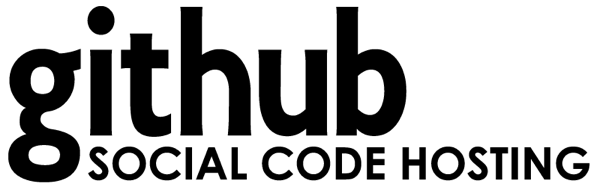
\includegraphics[width=0.2\textwidth]{github}
    
\includegraphics[width=0.2\textwidth]{git}
  \end{center}
\end{wrapfigure}
\textbf{Git} to otwarty rozproszony system kontroli wersji.
Pozwala na łatwe tworzenie i łączenie gałęzi rozwoju projektu, szybkie przemieszczanie się pomiędzy wersjami i sprawdzanie różnic pomiędzy nimi.
\textbf{Git} jest stosowany w takich projektach, jak jądro systemu Linux i umożliwia bardzo wiele (nawet w stosunku do innych nowoczesnych rozproszonych systemów kontroli wersji).
Niestety, powoduje to, że nie jest to system łatwy w nauce.

Zdecydowaliśmy się na system \textbf{Git}, ze względu na doskonały serwis \emph{Github}\footnote{\url{http://github.com}}

Serwis \emph{Github} posłużył nam nie tylko, jako przestrzeń do współdzielenia kodu.
Serwis ten udostępnia wiele narzędzi, które były bardzo przydatne w czasie prac nad projektem.
Korzystaliśmy z wykresów, które pomagały się zorientować, który członek zespołu co robi.
Inna przydatna opcja, z której korzystaliśmy, aby zapewnić wysoką jakość kodu, to komentowanie kodu napisanego przez innych.
Od kiedy został wprowadzony ulepszony system zadań (\emph{Issues 2.0}), korzystaliśmy z niego w celu przechowywania wymagań i komunikacji z opiekunem projektu.

Ponadto serwis pozwala na automatyczne powiadamianie o nowych zmianach w projekcie na kanale IRC, co było bardzo pomocne~--- motywowało do przeglądania kodu innych i usprawniało integrację.

\subsection{Inne narzędzia}
\subsubsection{Zintegrowane środowisko programistyczne}
W zespole nie zostało ustalone żadne środowisko programistyczne.
Część członków zespołu używała środowiska \emph{Eclipse}, część \emph{Netbeans}.

Niektórzy członkowie zespołu tworzyli kod za pomocą zwykłych edytorów tekstowych.

\subsubsection{Kanały komunikacji}
Głównymi kanałami komunikacji wewnątrz zespołu były rozmowy w rzeczywistości i na kanale IRC.

Ponadto, przez pewien czas korzystaliśmy z serwisu \emph{Scrumd}\footnote{\url{http://scrumd.com}}, służącego do zarządzania projektami prowadzonymi w metodyce Scrum.
Głównym zastosowaniem tego narzędzia było przechowywanie wymagań.
Wprowadzenie systemu \emph{issues 2.0} w serwisie \emph{Github} sprawiło, że serwis przestał być przydatny.

Korzystaliśmy także z serwisu \emph{piratepad}\footnote{\url{http://piratepad.net}}.
Serwis ten pozwala na jednoczesną edycję plików tekstowych i łatwe dzielenie się nimi.
Z serwisu korzystaliśmy we wczesnych wersjach projektu, kiedy ustalaliśmy ogólne cele i założenia.


  \section{Diagramy Klas}
    \begin{figure}
  \begin{center}
    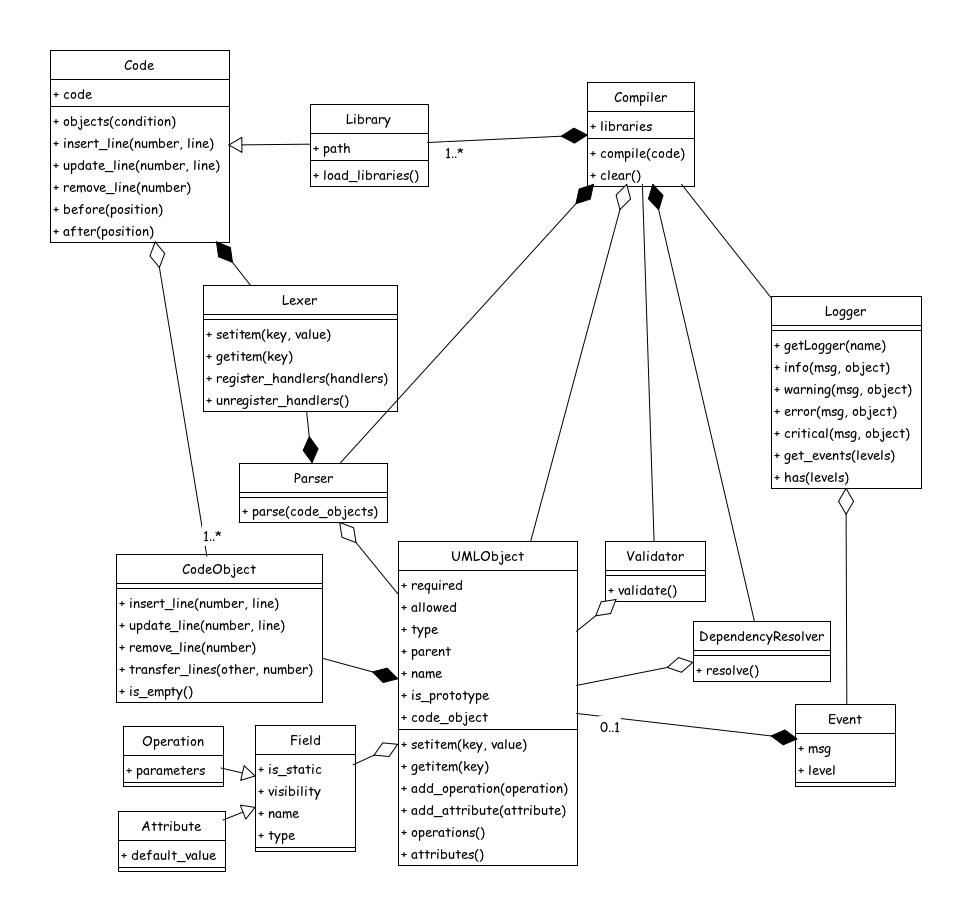
\includegraphics[width=\textwidth]{compiler}
  \end{center}
  \caption{Diagram klas modułu \texttt{compiler}}
\end{figure}

\begin{figure}
  \begin{center}
    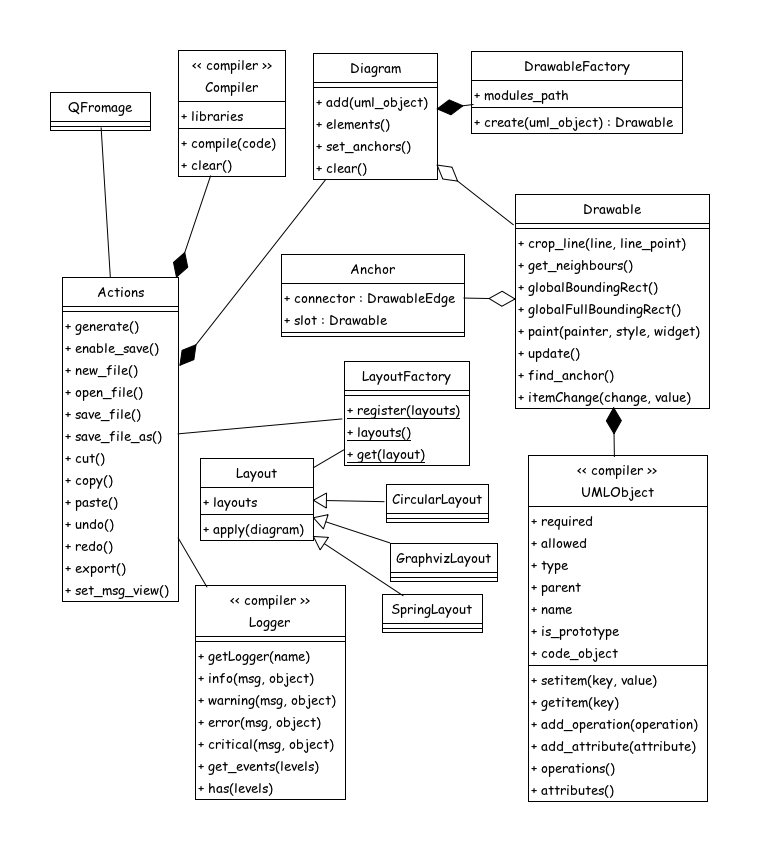
\includegraphics[width=\textwidth]{fromage}
  \end{center}
  \caption{Diagram klas modułu \texttt{fromage}}
\end{figure}

\begin{figure}
  \begin{center}
    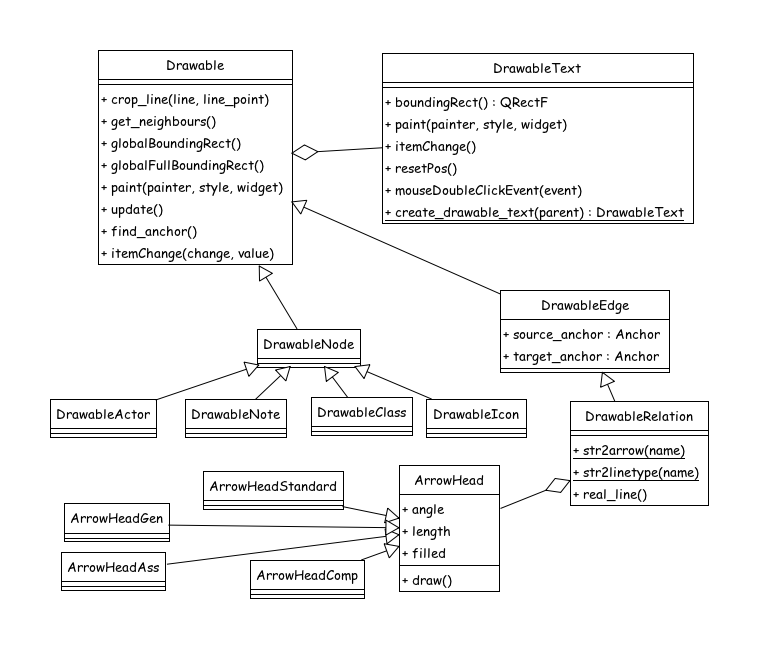
\includegraphics[width=\textwidth]{drawable}
  \end{center}
  \caption{Diagram klas modułu \texttt{modules}}
\end{figure}

  \section{Działanie programu}
    \subsection{Kompilacja}
      % subsection

Kompilacja diagramów w programie \omlet składa się z następującego zestawu czynności:

\begin{itemize*}
  \item{Wczytanie kodu i jego wstępny podział na obiekty}
  \item{Sparsowanie kodu}
  \item{Uzupełnienie obiektów danymi z ich prototypów}
  \item{Odrzucenie prototypów}
  \item{walidacja skompilowanych obiektów}
\end{itemize*}

\subsubsection{Wczytanie kodu}
Za ten etap odpowiedzialna jest klasa \texttt{Code}.
Klasa przyjmuje napis, zawierający plik źródłowy.
Za pomocą klasy \texttt{Lexer} sprawdzane są kolejne linie.
Jeżeli linia jest definicją obiektu, tworzony jest nowy obiekt typu \texttt{\_CodeObject}, zawierający linie należące do obiektu następującego po znalezionym nagłówku.
Poza samymi liniami \texttt{\_CodeObject} przechowuje także informacje pozwalające określić numery linii w źródle.

Ponieważ pierwszy wiersz źródła nie musi być nagłówkiem obiektu, tworzony jest specjalny obiekt zerowy, przechowujące wszystkie linie przed pierwszym obiektem.

\subsubsection{Parsowanie kodu}
Obiekt klasy \texttt{Code}, zawierający obiekty \texttt{\_CodeObject} jest następnie przesyłany do klasy \texttt{Parser}.
Klasa ta zawiera funkcje budujące obiekty klasy \texttt{UMLObject}, na podstawie rozpoznanych symboli.
Obiekt klasy \texttt{Parser} Tworzy obiekt klasy \texttt{Lexer}, w którym zdefiniowana jest gramatyka.

Następnie metody klasy \texttt{Parser}, służące do budowania obiektów \texttt{UMLObject} są dodawane jako obiekty obsługujące symbole gramatyki.
Ostatecznie metoda \texttt{parse\_string} klasy \texttt{Lexer} zostaje wywołana i zostają utworzone obiekty \texttt{UMLObject} odpowiadające plikowi źródłowemu.

\subsubsection{Uzupełnienie obiektów}
Za uzupełnienie obiektów odpowiada obiekt klasy \texttt{DependencyResolver}.
Obiekt ten otrzymuje wszystkie obiekty \texttt{UMLObject}, które zostały stworzone w poprzednich krokach (oraz obiekty biblioteczne, tworzone przy inicjalizacji kompilatora).

Na początku obiekt sprawdza, czy nie występują cykliczne zależności pomiędzy obiektami (t.j. czy dwa lub więcej obiektów nie jest wzajemnie swoimi prototypami).

Następnie dla każdego obiektu znajdowany jest obiekt, będący jego prototypem i właściwości tego obiektu są dopisywane do aktualnego obiekt (pod warunkiem, że obiekt sam takich właściwości nie określa).

Po dojściu do obiektu, którego prototypem jest \texttt{base}, uzupełnianie danej gałęzi obiektów zostaje zakończone.

\subsubsection{Odrzucanie prototypów}
Prototypy muszą być odrzucone z puli obiektów z dwóch powodów:
\begin{itemize*}
  \item{Nie powinny być rysowane na diagramie}
  \item{Nie muszą być spójne} (spełniać wszystkich wymagań określonych przez ich prototypy). Pozostawienie ich przed następnym krokiem spowodowałoby niepotrzebne błędy.
\end{itemize*}

\subsubsection{Walidacja obiektów}
Obiekt klasy \texttt{Validator} sprawdza zgodność z danymi walidacji określonymi przez jego prototypy.

Normalnie sprawdzane jest istnienie, bądź nie istnienie konkretnej właściwości obiektu, oraz ew. zgodność typu tej właściwości.
Jeżeli prototypy określają wymagane wartości o typie \texttt{Object}, to sprawdzane jest także, czy wskazane przez te wartości obiekty istnieją.

\end{document}
